
    \section{Frequenzgang der Gleichtaktverstärkung}
        Um nun die Gleichtaktverstärkung zu simulieren wird die Spannung von \(U_{V3}\) auf \SI{0}{\V} und die Spannung \(U_{V4}\) auf \SI{1}{\V} gesetzt.
        Somit sorgt dafür das \textbf{Eingang 1} und \textbf{Eingang 2} jeweils mit der gleichen Spannung versorgt werden. 
        \begin{figure}[ht!]
            \centering
            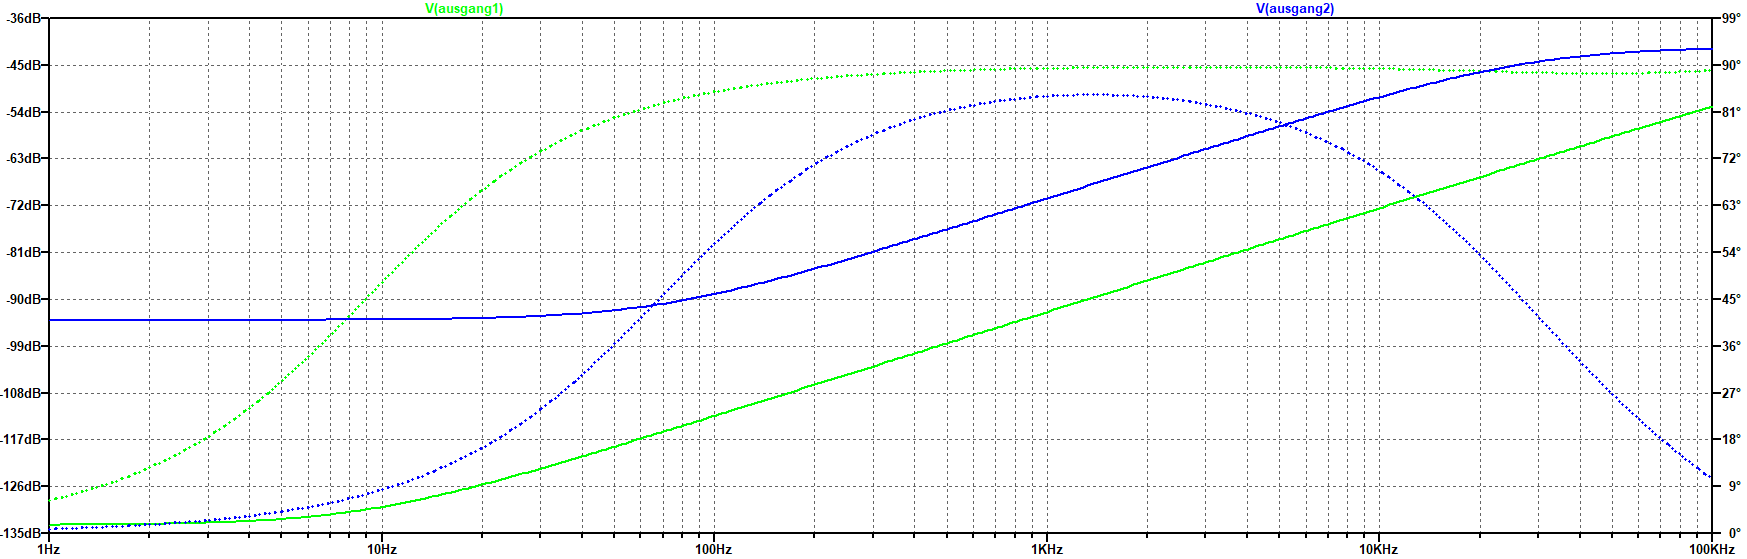
\includegraphics[width=\linewidth]{gleichtakt.png}
            \caption{Diagramm des Frequenzgangs Gleichtaktverstärkung}
        \end{figure}
        Bei einem Insturmentenverstärker liegt die niedrigste Gleichtaktfrequenz bei \(f=\SI{1}{\Hz}\). Mit hilfe der Curserfunktion wird nun die Verstärkung beider Ausgänge ausgelesen. 
        Für den Instrumentenverstärker aus drei Operationsverstärkern ergibt sich die niedrigste Gleichtaktverstärkung von \(v_{CM}=-\SI{133,371}{\dB}\) bei einer Frequenz von \(f=\SI{1}{\Hz}\)~\figref{gleichtaktwerte}.
        Für den integrierten Instrumentenverstärker ergibt sich die niedrigste Gleichtaktverstärkung von \(v_{CM}=-\SI{94,000}{\dB}\) bei einer Frequenz von \(f=\SI{1}{\Hz}\).
        Aus den Datenblätter lassen sich die Werte für die Gleichtaktunterdrückung \(v_{cmrr}\) entnehmen.
        \begin{table}[h!]
            \centering
            \caption{Ergebnisse der Gleichtaktverstärkung über den Frequenzgang}
            \begin{tabular}{|c|c|c|}
                \hline
                für \(f=\SI{1}{\Hz}\)  & Sim. \(v_{CM}\) & \(v_{cmrr}\) der Datenblätter\\ \hline 
                TL084 & \(\SI{-133,371}{\dB}\)&\(\SI{86}{\dB}\)\\ \hline
                AD8226 & \SI{-94,000}{\dB}&\(\SI{120}{\dB}\)\\ \hline
            \end{tabular}
        \end{table}
        Der Instrumentenverstärker aus drei Operationsverstärkern hat eine geringe Gleichtaktverstärkung bei \(f=\SI{1}{\Hz}\), dieser Wert ist deutlich niedriger als der Wert aus dem Datenblatt. Ursache hierfür ist die Tatsache das mehrere Operationsverstärker vom Typ TL084 verbaut sind. 
        Hinzu zufügen ist das der Wert \(v_{cmrr}=\SI{86}{\dB}\) kein maximal Wert ist.\par
        Der integrierte Instrumentenverstärker liefert laut Datenblatt eine Gleichtaktunterdrückung von minimal \(v_{cmrr}=\SI{120}{\dB}\) und bei Frequenzen \(f>\SI{5}{\Hz}\) eine Unterdrückung von \(v_{cmrr}=\SI{90}{\dB}\). Dies stimmt mit der Simulation nur bedingt überein. \par
        Bei beiden Integrationsverstärker sieht man mit zunehmender Frequenz eine stetig wachsende Verstärkung. Der Grund hierfür liegt daran, dass reelle Instrumentenverstärker simuliert werden und diese in ihren Operationsverstärkern zum Eingang eine parallel geschaltete parasitäre Kapazität besitzen. 
        Die hat eine negative Auswirkung auf die Gleichtaktunterdrückung, da sie mit steigender Frequenz zunehmend leitend wirken. 
        
        \begin{figure}[ht!]
            \centering
            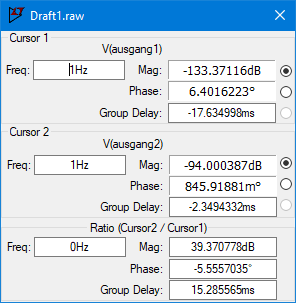
\includegraphics[]{gleichtaktwert.PNG}
            \caption{Gleichtaktverstärkung von Ausgang 1 und 2}
            \label{gleichtaktwerte}
        \end{figure}
        \newpage
    \section{Einfluss von Widerstandstoleranzen}
        Um den Einfluss zu messen, den ein Widerstand mit einer Toleranz von \(\pm \SI{1}{\ohm}\) hat, wird der Wert von \(R_6\) um \SI{1}{\percent} gesenkt.
        Hierbei ergibt sich ein neuer Wert für von \(R_6= \SI{33}{\kilo\ohm}\cdot 0,99 = \SI{32,670}{\kilo\ohm}\). Die Simulation wird mit dem abgeänderten Wert von \(R_6\) durchgeführt. Am \textbf{Ausgang 1} kann man folgenden Graf ablesen.
        \begin{figure}[ht!]
            \centering
            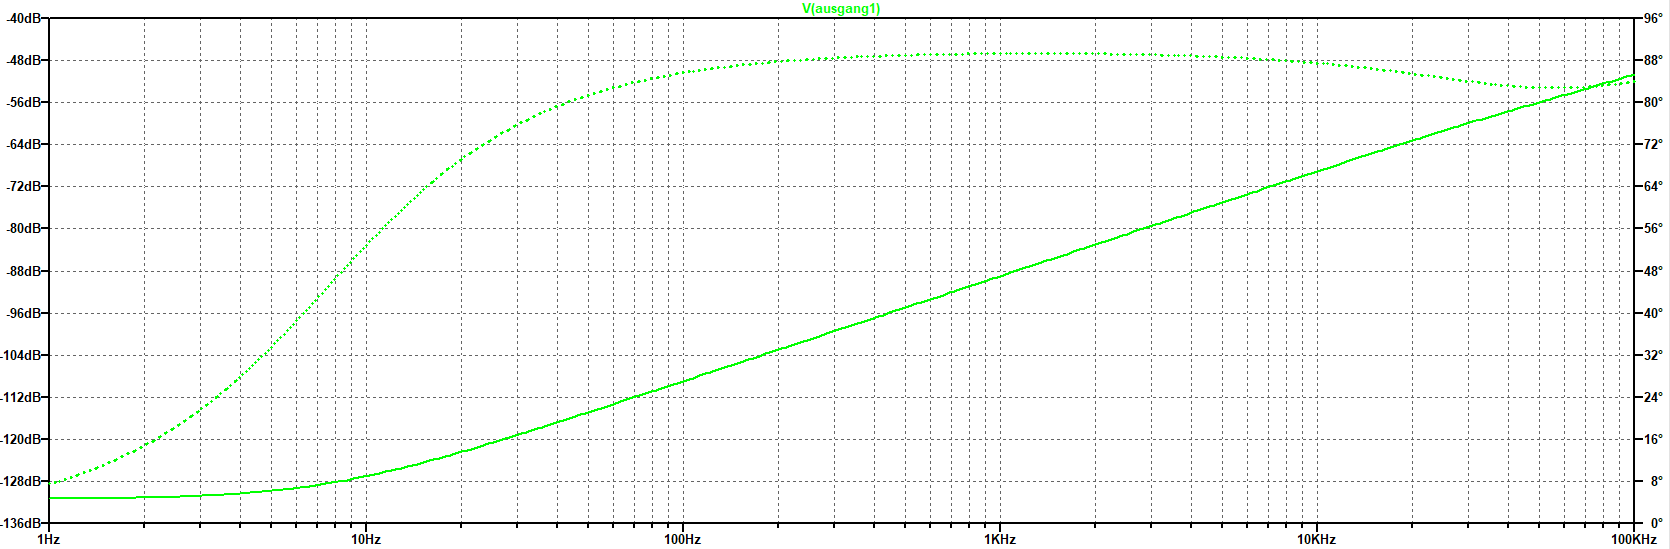
\includegraphics[width=\linewidth]{widerstandr6.PNG}
            \caption{Graf der Schaltung mit verändertem R6}
        \end{figure}
        Auch hier wird mit hilfe der Curserfunktion der Wert \(f=\SI{1}{\Hz}\) abgelesen. Hier kann man ein Wert von \(v_{tol1} = -\SI{133,237}{\dB}\) sehen. \par
        Um die Auswirkung einer Toleranz von \SI{1}{\percent} zu sehen werden alle Werte der Widerstände 1-7 um die Toleranz geändert~\figref{toleranzschaltung}. 
        \begin{figure}
            \centering
            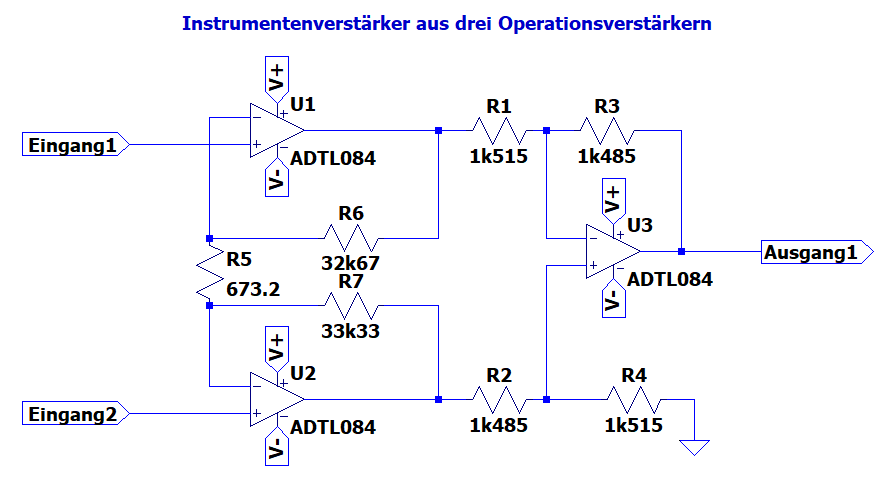
\includegraphics[width=\linewidth]{maxtoleranz.PNG}
            \caption{Schaltung mit allen Widerständen um \(\pm\SI{1}{\percent}\) geändert}
            \label{toleranzschaltung}
        \end{figure}
        Wird nun die Simulation gestartet erhält man den Frequenzgang aus ~\ref{toleranzgraf}.
        \begin{figure}[ht!]
            \centering
            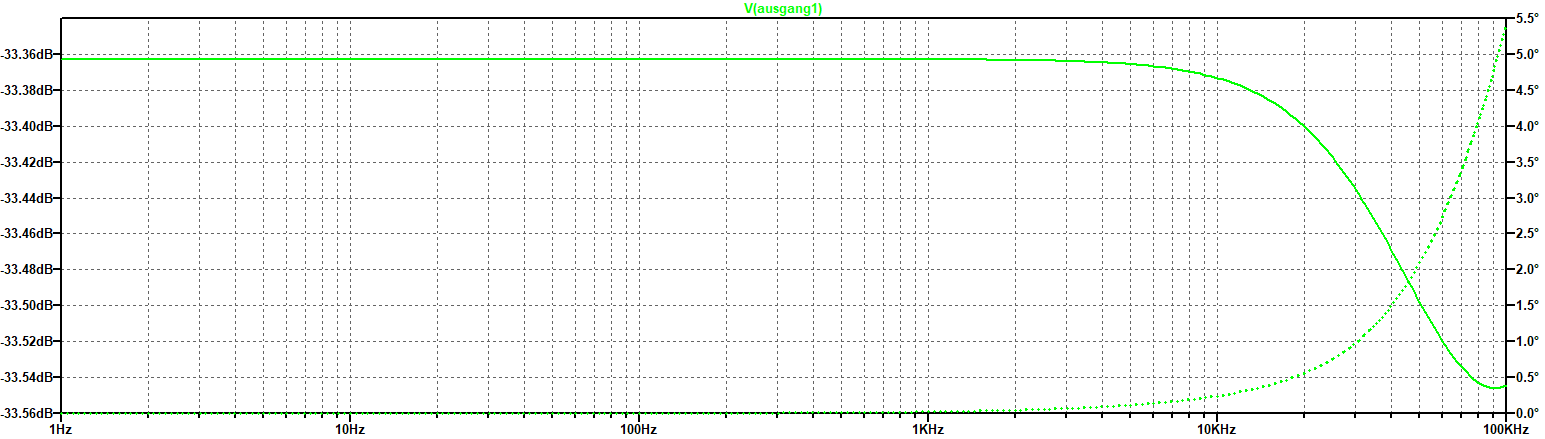
\includegraphics[width=\linewidth]{toleranzwerte.PNG}
            \caption{Gleichtaktverstärkung mit veränderten Widerstandstoleranzen}
            \label{toleranzgraf}
        \end{figure}

        \begin{table}[h!]
            \centering
            \caption{Ergebnisse der Gleichtaktverstärkung über den Frequenzgang}
            \begin{tabular}{|c|c|c|c|}
                \hline
                für \(f=\SI{1}{\Hz}\)  & indeale Widerstände & \(R_6\) mit Toleranz der Datenblätter & alle R mit Toleranz\\ \hline 
                \(v_{CM}\) in dB & \(\SI{-133,371}{\dB}\)&\(-\SI{133,237}{\dB}\)&\(-\SI{33,363}{\dB}\)\\ \hline
            \end{tabular}
        \end{table}
        Hierbei zeigt sich das wenn nur ein Wiederstand (\(R_6\)) vom Idealwert abweicht, die Veränderung quasi Null ist. Auch wenn man andere Widerstände einzeln verändert, wirkt es sich quasi garnicht auf die Verstärkung aus. 
        Werden alle Widerstände jedoch verändert, hat dies große Auswirkungen auf die Gleichtaktunterdrückung. Diese steigt stark an und damit sinkt die Gleichtaktverstärkung. 
